\setcounter{secnumdepth}{-1}

\chapter{Synchronization errors}

\section{Description}

Because the receiver and transmitter are not at the same location, the carrier frequencies and the samplers at TX and RX will have a different phase and due to the inaccuracies of the oscillator, the frequencies will also be slightly different. \\
This is summarized in 4 effects:
\begin{itemize}
    \item \textbf{Carrier frequency offset (CFO)}: The difference in the carrier frequencies at TX and RX ($=\Delta \omega$). It will add ISI as the RRC are not anymore matched and a linearly increasing phase shift will appear.
    \item \textbf{Phase offset}: The difference between the phase of the carrier signal at TX and RX.
    \item \textbf{Sampling frequency offset (SFO)}: The difference in the sampling frequencies at TX and RX.
    \item \textbf{Time shift}: The difference in the timing of the samples at TX and RX.
\end{itemize}

\section{Implementation}

\subsection{CFO}
The CFO implementation is done by multiplying the signal with a complex exponential $e^{j2\pi \phi_{\text{ppm}}f_c t}$. The phase offset is added to the CFO. It is defined in ppm (part per million) where the ppm value is $\frac{\Delta\omega}{f_c} 10^{-6}$. \\
Figure \ref{fig:CFO_BER} shows the BER curves with different CFO values. In order to have useful results, the linear phase shift is removed right after the second RRC filter. This allows to only keep the effect of ISI on the BER curve.

\begin{figure}[H]
    \centering
    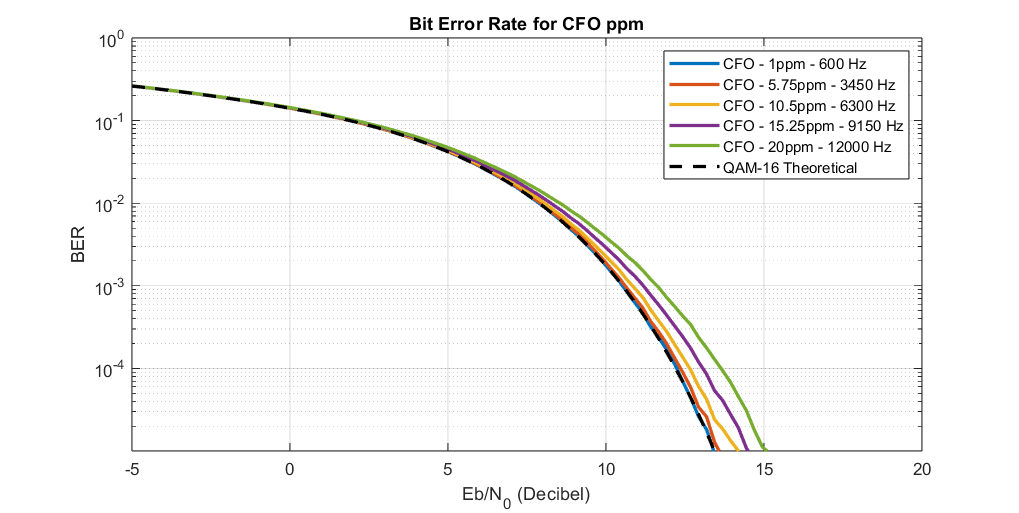
\includegraphics[width=0.8\textwidth]{CFO_ppm.png}
    \caption{BER with different CFO values}
    \label{fig:CFO_BER}
\end{figure}

Figure \ref{fig:CFO_const} shows the effect of CFO on the symbol constellation for QAM-16. It is here plotted without any noise and with parameters that allow us to see the line phase shift of the symbols. \\

\begin{figure}[H]
    \centering
    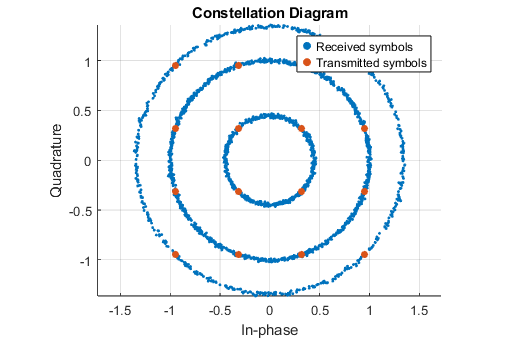
\includegraphics[width=0.8\textwidth]{constellation_CFO.png}
    \caption{Constellation before and after CFO}
    \label{fig:CFO_const}
\end{figure}

\subsection{Phase offset}
The same is done for the phase offset where the exponential is simply $e^{j\phi}$ where $\phi$ is chosen once at the begining of the simulation. \\

The effect of the phase offset is only visible on the constellation plot (figure \ref{fig:phaseOffsetConst}) where every point is rotated by a fixed angle (whereas CFO rotated the symbols linearly with time). \\

\begin{figure}[H]
    \centering
    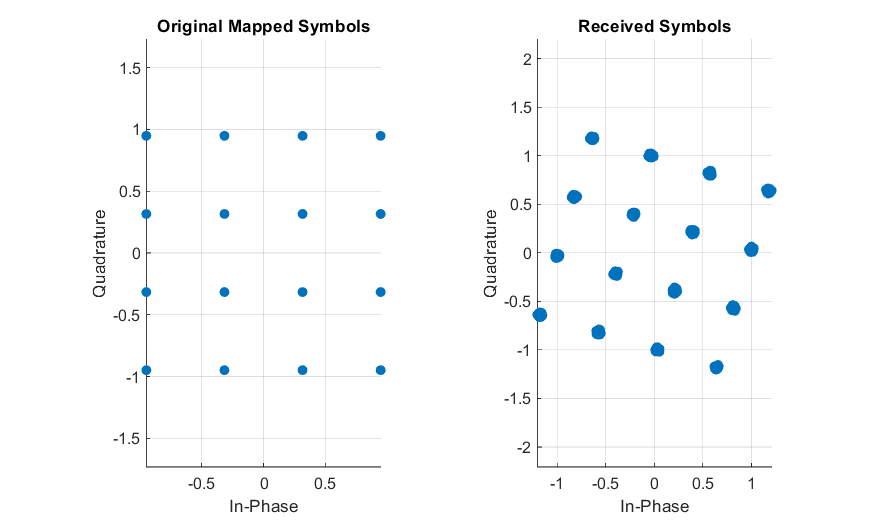
\includegraphics[width=0.8\textwidth]{constellation_carrier_offset.png}
    \caption{Constellation before and after phase offset}
    \label{fig:phaseOffsetConst}
\end{figure}

On a BER curve (figure \ref{fig:BER_PO}), the phase is not visible as from the errors originating from the phase offset are either on every symbol or on none and this is why the error does not depend anymore on $E_b/N_0$. \\

\begin{figure}[H]
    \centering
    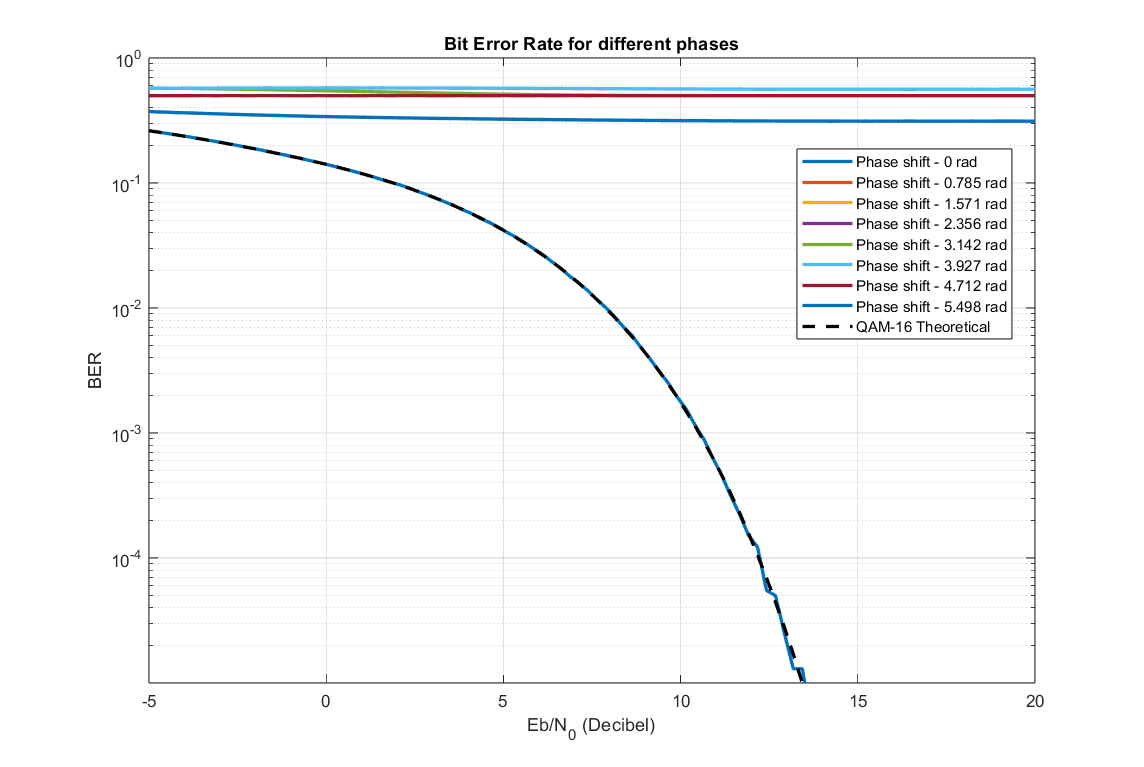
\includegraphics[width=0.8\textwidth]{BER_PO.png}
    \caption{BER with phase offset}
    \label{fig:BER_PO}
\end{figure}

\subsection{SFO}
The SFO is neglected in the simulation as it would need some interpolation and more complex computations. \\

\subsection{Time shift}
The time shift is implemented by simply shifting the samples in the array with an oversampling factor that is large enough. \\
A larger time shift will increase the BER as the samples will be taken at the wrong time. For sufficiently low values, it will still behave as a "classical" BER curve but from some point, there is just no more correlation between the measured sample and the received one and the BER tends to a $0.5$ line, as shown in figure \ref{fig:BER_TS}. \\

\begin{figure}[H]
    \centering
    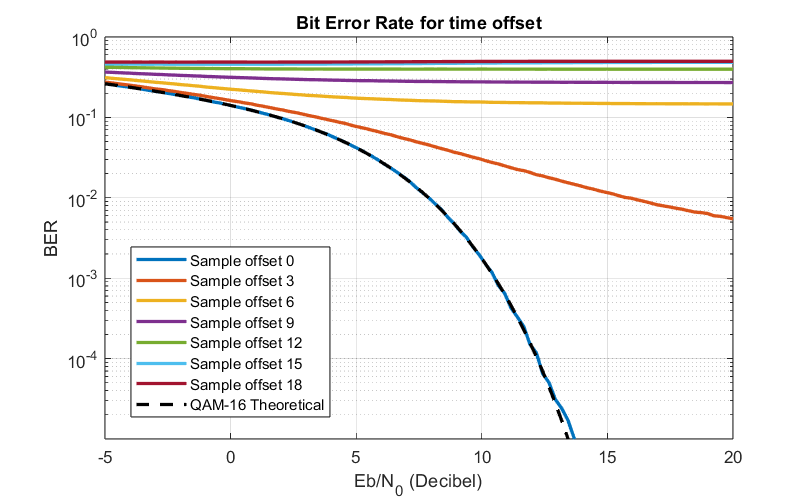
\includegraphics[width=0.8\textwidth]{BER_TS.png}
    \caption{BER with time shift}
    \label{fig:BER_TS}
\end{figure}

\section{Correction}

\subsection{Frame and frequency acquisition}

With the previous correction, the receiver knows when to sample but there still is some uncertainty on the frequency. The way to remove the CFO is to send in the data a known pilot and the first step is to detect when this pilot is received. This is known as frame acquisition and it is performed with the differential cross-correlator:

\begin{equation*}
    D_k[n] = \frac{1}{N-k} \sum_{l=k}^{N-1} \left(y^*[n+l]a[l]\right) \left(y^*[n+l-k]a[l-k]\right)^*
\end{equation*}

Where $a$ is the known pilot, $N$ its length and $k$ the delay between the two correlations. \\
$D_k[n]$ is computed for every time index $n$ and for every shift $k$ until its maximum value, $K$. The estimation of the index of the start of the frame $\hat{n}$ and the estimation of the CFO $\hat{\Delta f}$ are given by:

\begin{equation*}
    \hat{n} = \text{arg} \max_n \sum_{k=1}^{K} |D_k[n]|
\end{equation*}
\begin{equation*}
    \hat{\Delta f} = -\frac{1}{K} \sum_{k=1}^{K} \frac{\angle D_k[\hat{n}]}{2\pi kT}, \qquad T \text{ being the symbol duration.}
\end{equation*}

The implementation of the time of arrival estimator has been done on figure \ref{fig:TOA_demo} by placing the pilot at the 100th sample and by then plotting $\sum_{k=1}^{K} |D_k[n]|$. The peak at the 100th sample clearly indicates the time of arrival of the pilot and validates the implementation. A similar test was done for the CFO estimation but it is not shown here. \\

\begin{figure}[H]
    \centering
    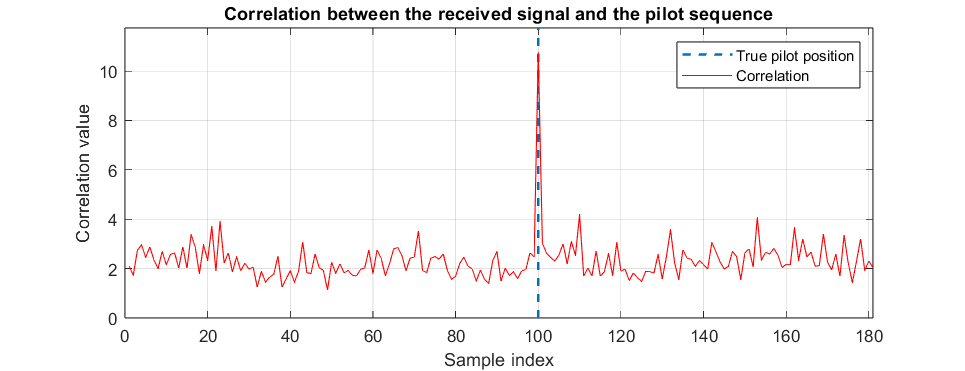
\includegraphics[width=1\textwidth]{TOA_demo.png}
    \caption{Time of arrival estimation}
    \label{fig:TOA_demo}
\end{figure}

The standard deviation of both estimators has been mesured on 250 runs for both a varying pilot length $N$ and a varying maximal shift $K$ for an increasing $\frac{E_b}{N_0}$ in figures \ref{fig:TOA_CFO_std_N} and \ref{fig:TOA_CFO_std_K}. 

\begin{figure}[H]
    \centering
    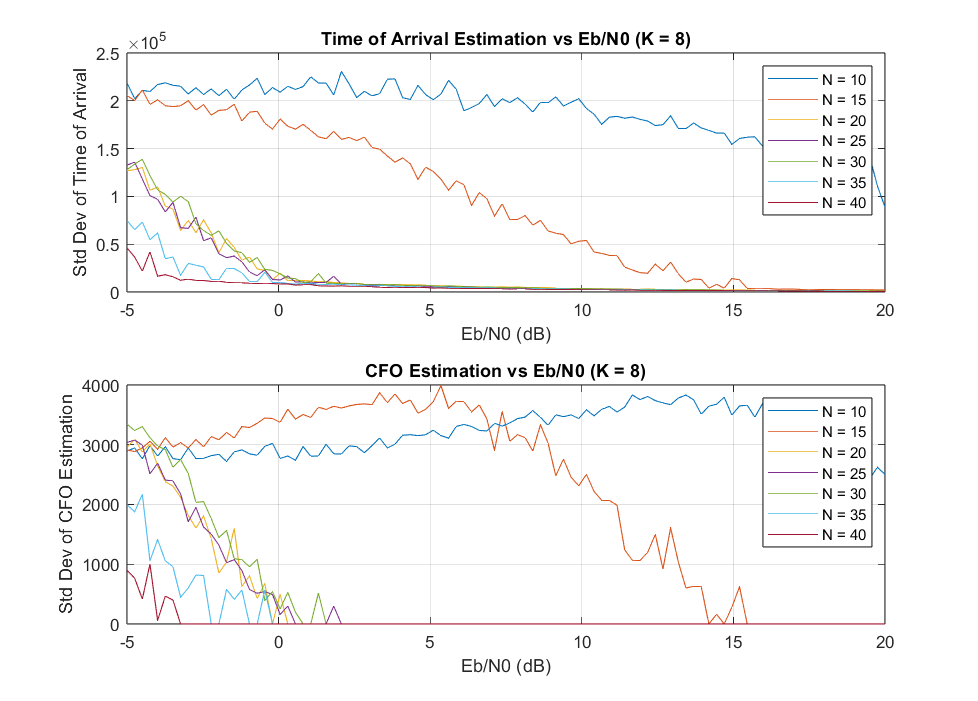
\includegraphics[width=1\textwidth]{TOA_CFO_std_56m.png}
    \caption{Standard deviation of the CFO estimator with varying pilot length}
    \label{fig:TOA_CFO_std_N}
\end{figure}

\begin{figure}[H]
    \centering
    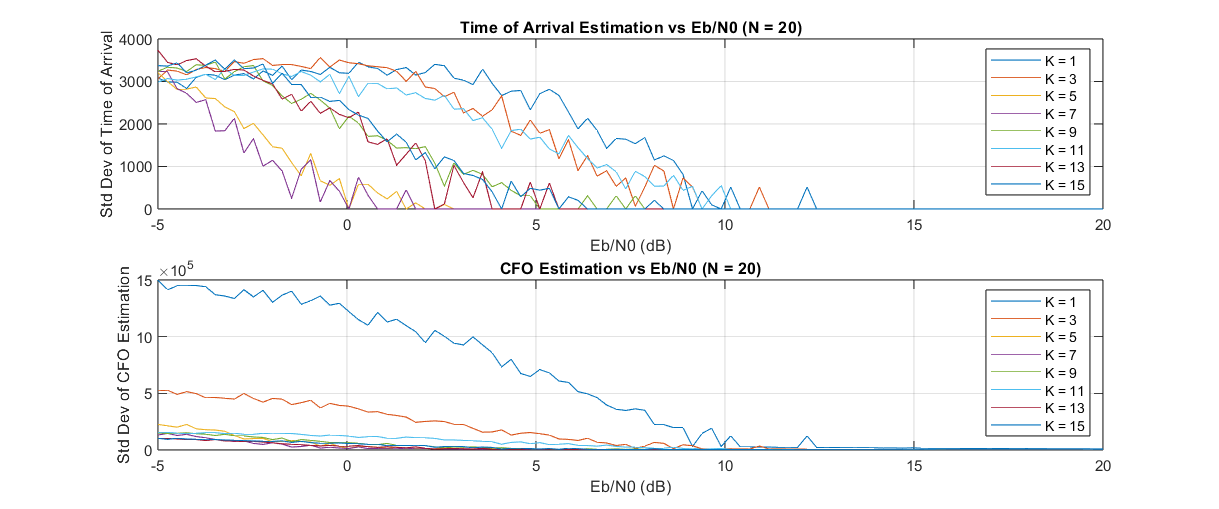
\includegraphics[width=1\textwidth]{TOA_CFO_std_K_56m.png}
    \caption{Standard deviation of the CFO estimator with varying maximal shift}
    \label{fig:TOA_CFO_std_K}
\end{figure}

As expected, a longer pilot and a larger shift will lower the uncertainty of the estimation and the same goes by for an increasing SNR. The fact that the line corresponding to $N = 10$ on figure \ref{fig:TOA_CFO_std_N} does not seem to decrease with $\frac{E_b}{N_0}$ is explained by the fact that $N$ and $K$ are too close to each other.\\
The robustness of the frame acquisition is also tested against a varying CFO.
